\chapter{Comportamiento longitudinal}
\label{ch:longitudinal-model}

El comportamiento longitudinal es un problema de regresión sobre cómo ha de comportarse la aceleración del \gls{dvu}\index{driver-vehicle unit} en función de la información existente alrededor. Los perfiles de aceleración para los conjuntos de entrenamiento y de test se ilustran en la Figura~\ref{fig:acceleration-profiles}.

\begin{figure}
	\centering
	\subfloat[Entrenamiento]{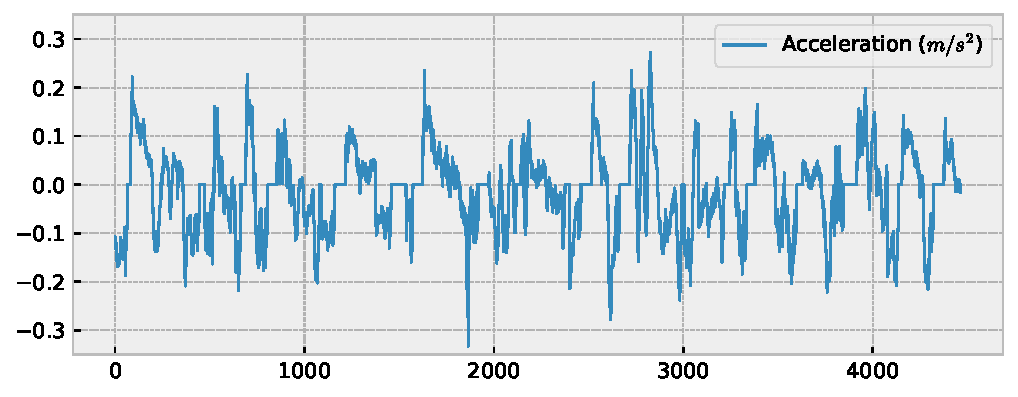
\includegraphics[width=\textwidth]{acceleration-profiles-training}}\qquad
	\subfloat[Test]{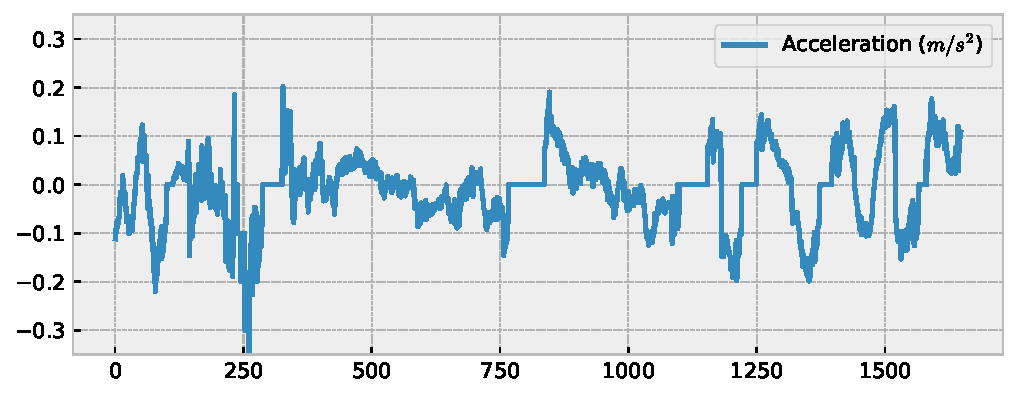
\includegraphics[width=\textwidth]{acceleration-profiles-test}}
	\caption[Perfiles de aceleración a ajustar por los modelos. Conjuntos de entrenamiento y de test]{Perfiles de aceleración durante los experimentos: (a) entrenamiento y (b) test. Estos son los conjuntos de datos que se intentarán ajustar con los modelos.}
	\label{fig:acceleration-profiles}
\end{figure}

Por la naturaleza del problema se han seleccionado dos técnicas diferentes para el ajuste del modelo:

\begin{enumerate}
	\item \Acrshort{mlp}\index{perceptron multicapa}. Al ser un problema de regresión, el uso de \acrlongplsp{mlp} en el comportamiento longitudinal está justificado al ser considerados éstos aproximadores universales\sidenote{
			El \textit{Teorema de aproximación Universal} \cite{hornik1991approximation} postula que un \acrlongsp{mlp}\index{perceptron multicapa} con al menos una capa oculta es capaz de aproximar cualquier función si dispone de suficientes neuronas en ésta.
	}.
	\item \Acrshort{fcs}\index{sistema de control borroso}. La formulación del problema se ajusta muy bien al funcionamiento de estos modelos. Además, los \acrlongplsp{fcs}\index{sistema de control borroso} tienen la ventaja de que se puede explicar su funcionamiento, a diferencia de los \acrlongplsp{mlp}\index{perceptron multicapa} con una o más capas ocultas.
\end{enumerate}

Ambos modelos se ajustarán con un procedimiento basado en el descenso del gradiente denominado ADAM~\cite{kingma2014adam}. Su aplicación a los \acrlongplsp{mlp}\index{perceptron multicapa} es directa (después de todo es una técnica desarrollada dentro de área de las \acrlongplsp{ann}\index{red neuronal artificial}), pero para los \acrlongplsp{fcs}\index{sistema de control borroso} es necesaria una representación que permita el uso de este método para su optimización. Esta representación es una de las aportaciones de esta tesis y se se explica en el apéndice \nameref{ch:fuzzy-controller-adjustment}.

El error que se trata de minimizar es el cuadrado del \gls{rmse}\index{RMSE} entre los valores de aceleración del conjunto real y los ajustados por el modelo. Los resultados no obstante se presentan con el \gls{rmse}\index{RMSE} ya que éste es directamente interpretable en las medidas de la variable sobre la que se aplica (en nuestro caso, \SI{}{\metre\per\square\second}).

\section{Descripción de los datasets}

Del conjunto de datos descrito en la Tabla~\ref{tbl:main-variables} del capítulo~\nameref{ch:methodology} seleccionamos aquellos indicadores de interés: \textit{Distancia a líder}, \textit{Distancia a siguiente TLS}, \textit{Estado de siguiente TLS}, \textit{Velocidad}, \textit{Velocidad a líder} y \textit{Aceleración} (este último como salida a ajustar por el modelo). Estos valores conformarán los conjuntos de entrenamiento y de test tanto para cada uno de los sujetos $S_1$, $S_2$ y $S_3$, como para el conjunto global de éstos $S_A$.

Dado que nuestros modelos se basan en un esquema \textit{\idx{feed-forward}}, existe el inconveniente de que para ellos es imposible mantener una memoria del orden en el que se están sucediendo las entradas. Sin embargo, contamos con las derivadas de la posición respecto al líder (la aceleración y la velocidad al líder) y la velocidad, por lo que consideramos que disponemos de información temporal suficiente para este problema en concreto.

El resultado de la generación de los datasets de entrenamiento y test para todos los sujetos se resume en la Tabla~\ref{tbl:cf-datasets-description}

\begin{table}
	\centering
	\caption[Descripción de los conjuntos de datos]{Descripción de los conjuntos de datos para el entrenamiento de los modelos. $CF_{S_A}$ se corresponde con el modelo de conductor global, mientras que cada $CF_{S_i}$ es la porción de datos correspondiente al sujeto $S_i$.}
	\label{tbl:cf-datasets-description}
	\begin{tabularx}{\textwidth}{YYYYY}
		\toprule
		& & & \multicolumn{2}{c}{Tamaño} \\
		& Entradas & Salidas & Entrenamiento & Test \\
		\midrule
		\rowcolor{black!20} $CF_{S_1}$ & $7$ & $1$ & $1089$ & $543$ \\
		$CF_{S_2}$ & $7$ & $1$ & $1313$ & $560$ \\
		\rowcolor{black!20} $CF_{S_3}$ & $7$ & $1$ & $2067$ & $668$ \\
		$CF_{S_A}$ & $7$ & $1$ & $4469$ & $1771$ \\
		\bottomrule
	\end{tabularx}
\end{table}

\section{Modelo basado en \acrlongplsp{fcs}\index{sistema de control borroso}}

Se han realizado entrenamientos sobre arquitecturas con diferente número de particiones borrosas en las variables. Las arquitecturas que se han considerado más relevantes (tras un proceso de ensayo y error con diferente número de particiones borrosas) se describen en la Tabla~\ref{tbl:cf-fcs-architectures}. 

\begin{table*}
	\centering
	\caption[Resumen de las arquitecturas \ac{fcs}\index{sistema de control borroso} para el modelo longitudinal][2em]{Resumen de las arquitecturas seleccionadas. La posición de cada número de la arquitectura indica a qué variable lingüística se refiere (\textit{Distancia al líder}, \textit{Distancia a siguiente TLS}, \textit{TLS en verde}, \textit{TLS en amarillo}, \textit{TLS en rojo}, \textit{Velocidad} y \textit{Velocidad de aproximación al líder} respectivamente). Su valor se corresponde al número de conjuntos borrosos de la partición de cada una de ellas.}
	\label{tbl:cf-fcs-architectures}
	\begin{tabularx}{\linewidth}{XXXXXX}
		\toprule
		\multirow{2}{*}{} & \multirow{2}{*}{Arquitectura} & \multirow{2}{*}{Epochs} & \multicolumn{3}{c}{RMS}      \\ 
		& & & Entrenamiento & Validación & Test \\
		\midrule
		\rowcolor{black!20} $FCS_1$ & $2, 2, 2, 2, 2, 2, 2$ & $10^5$ & $0.059$ & $0.064$ & $0.062$  \\
		$FCS_2$ & $3, 3, 2, 2, 2, 3, 3$ & $10^5$ & $0.073$ & $0.079$ & $0.080$  \\
		\rowcolor{black!20} $FCS_3$ & $4, 3, 2, 2, 2, 3, 3$ & $10^5$ & $0.072$ & $0.078$ & $0.088$  \\
		$FCS_4$ & $5, 5, 2, 2, 2, 5, 5$ & $10^5$ & $0.063$ & $0.068$ & $0.109$  \\
		\bottomrule
	\end{tabularx}
\end{table*}

Todas las arquitecturas mantienen el número de conjuntos borrosos\index{conjunto borroso} asociados a las variables de estado del semáforo (verde, ámbar y rojo) a $2$. La razón es debido a que dicha variable sólo puede tomar dos valores, $0$ o $1$, y en la inicialización de sus respectivas particiones, estas variables ya toman dichos valores con un grado de pertenencia de $1$ en sus dominios.

Cada uno de los controladores se ha entrenado durante $250000$ \textit{epochs}\index{epoch}. En la Figura~\ref{fig:lm-fcs-rmse-all-comparisons} se puede observar la evolución en general y un detalle de la disminución del error durante el entrenamiento de los controladores. El error en test se ofrece a título informativo, y no ha sido usado para determinar las arquitecturas seleccionadas.

\begin{figure}
	\centering
	\subfloat[Entrenamiento y validación]{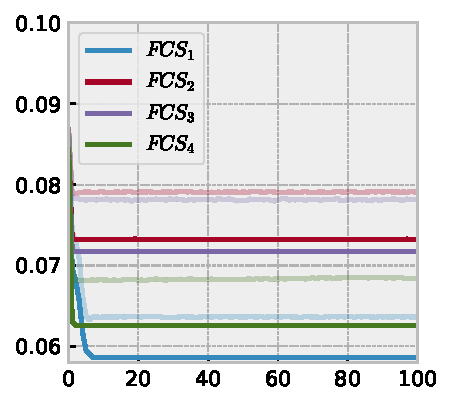
\includegraphics[width=.45\textwidth]{lm-fcs-rmse-all-training-and-validation-detail}}\qquad
	\subfloat[Test]{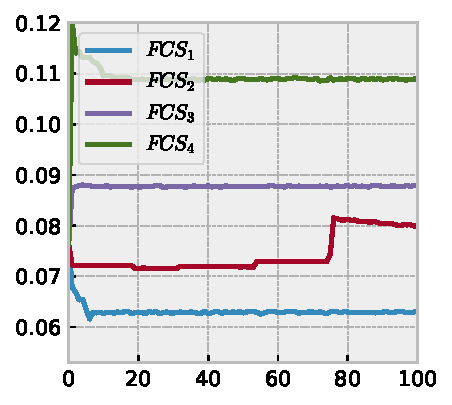
\includegraphics[width=.45\textwidth]{lm-fcs-rmse-all-test-detail}}
	\caption[Evolución del error durante el entrenamiento en las arquitecturas de \acrshort{fcs} para el modelo longitudinal]{Visión en detalle de la evolución del error en los conjuntos de entrenamiento y validación (izquierda) y de test (derecha). Para cada arquitectura, el color más transparente se corresponde al error en el conjunto de validación. El error de test se muestra debido a que nos ofrece puede ofrecer intuición de qué forma aprende la red, pero su evolución no se ha considerado para determinar las arquitecturas.}
	\label{fig:lm-fcs-rmse-all-comparisons}
\end{figure}

En un principio, el proceso de entrenamiento ha sido el habitual, ajustando todas las variables a la vez (particiones borrosas y pesos asociados a las reglas). Sin embargo, tras varias pruebas, se ha comprobado que el ajuste de las variables que determinan las particiones borrosas parece suceder más rápido que el ajuste de los pesos asociados a las reglas.

Por ello, en lugar entrenar a la vez, se ha particionado el entrenamiento en secuencias sucesivas de entrenamiento de reglas y entrenamiento de particiones borrosas.

Concretamente, los $250000$ epochs de entrenamiento han sido divididos en $250$ iteraciones de:

\begin{enumerate}
	\item $800$ epochs ajustando sólo las reglas con una tasa de entrenamiento de $0.01$.
	\item $200$ epochs ajustando sólo las variables de las particiones borrosas con una tasa de entrenamiento de $0.001$.
\end{enumerate}

Empíricamente (y para este problema en concreto) se ha podido observar que el entrenamiento realizado de esta manera hace que el \ac{rmse} descienda más rápido en el mismo número de iteraciones.

Se puede observar que la arquitectura $FCS_1$ es la que mejor error en test ha alcanzado. En las pruebas realizadas para el ajuste de controladores se ha observado además que los errores en entrenamiento y en test tienden a ser similares cuando los problemas son representables con un \acrlongsp{fcs}\index{sistema de control borroso}.

Éste será por tanto, el modelo seleccionado para la comparativa final. Las funciones de pertenencia ajustadas se muestran en la Figura~\ref{fig:adjusted-fuzzy-partitions} contrastadas con las versiones de antes de comenzar el entrenamiento, donde $f_i$ se corresponde con la función de pertenencia que caracteriza al conjunto borroso $i$-ésimo de la variable. Las reglas, sin embargo, son muy numerosas para ser incluidas en el texto, ya que la mayoría de reglas posibles en el sistema (aproximadamente $60$) tienen un peso asociado de más de $0.5$.

\begin{figure}
	\centering
	\subfloat[Distancia a líder]{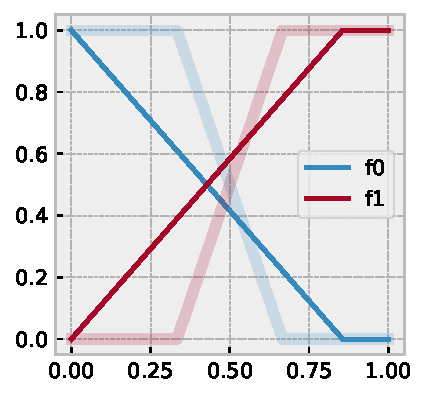
\includegraphics[width=.45\textwidth]{lm-fcs-best-architecture-leader-distance-variable-partition}}\qquad
	\subfloat[Distancia a siguiente semáforo]{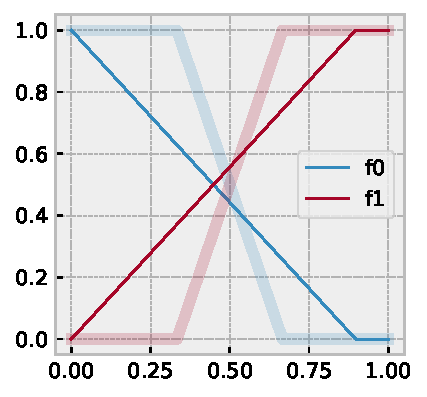
\includegraphics[width=.45\textwidth]{lm-fcs-best-architecture-next-tls-distance-variable-partition}}\qquad
	\subfloat[Velocidad]{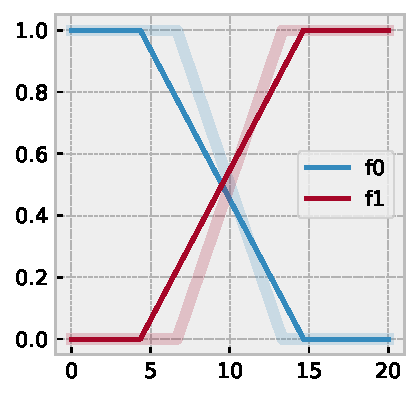
\includegraphics[width=.45\textwidth]{lm-fcs-best-architecture-speed-variable-partition}}\qquad
	\subfloat[Velocidad a líder]{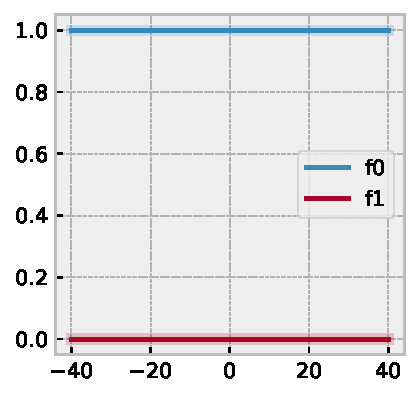
\includegraphics[width=.45\textwidth]{lm-fcs-best-architecture-speed-to-leader-variable-partition}}
	\caption[Particiones borrosas después de la operación de ajuste en el modelo longitudinal basado en \acrshort{fcs}]{Particiones borrosas después de la operación de ajuste en el modelo longitudinal basado en \acrshort{fcs}.}
	\label{fig:adjusted-fuzzy-partitions}
\end{figure}

Las funciones de pertenencia correspondientes al estado del semáforo no se incluyen ya que no se vieron modificadas en ningún entrenamiento. Después de todo, estas variables eran binarias, y las particiones borrosas se inicializan de tal manera que dichos valores siempre alcanzan un valor de pertenencia $1$.

Un detalle que merece la pena destacar es el aprendizaje de la variable lingüística \textit{Velocidad a Líder}. En todos los entrenamientos conducidos con las arquitecturas de la Tabla~\ref{tbl:cf-fcs-architectures} el comportamiento ha sido el mismo, es decir, que un único conjunto difuso cubra todo el dominio de la variable. Además, todas las reglas de activación han tenido dicho conjunto en cuenta, lo que da indicios de que dicha variable tiene un efecto mínimo o nulo sobre el comportamiento longitudinal. Sin embargo, de acuerdo a la literatura, prácticamente todos los modelos se basan en la diferencia de velocidad entre vehículos (extraída empíricamente), por lo que la explicación no puede ser esa. La explicación más plausible que podemos encontrar a dicho efecto es que, al tratarse de un entorno urbano, las velocidades que tratamos son muy bajas en comparación con las que se trabaja en este tipo de modelos, y por tanto, la diferencia de velocidades no son un factor determinante en comparación con el resto de variables.

En la Figura~\ref{fig:fcs-test-comparisons} se muestran los perfiles de la aceleración estimada por los controladores frente la aceleración real en cada momento. 

\begin{figure}
	\centering
	\subfloat[Perfil de aceleración]{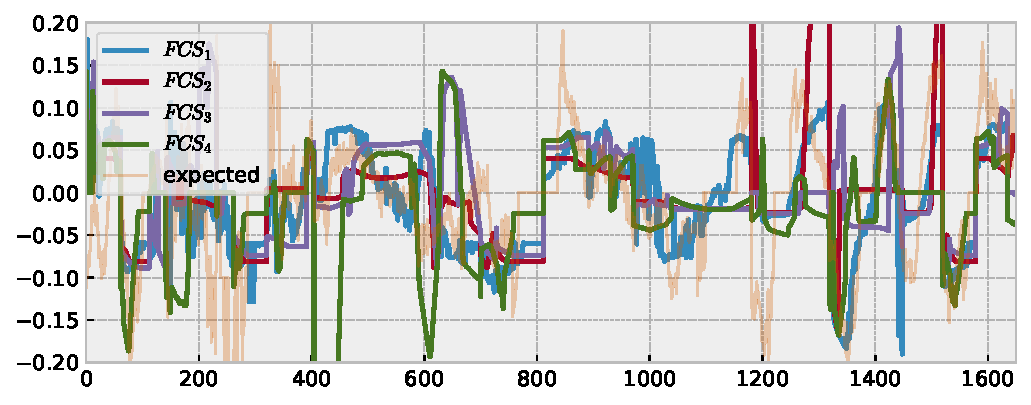
\includegraphics[width=\textwidth]{lm-fcs-outs-all-test-comparison}}\qquad
	\subfloat[Detalle entre frames de $750$ a $1050$]{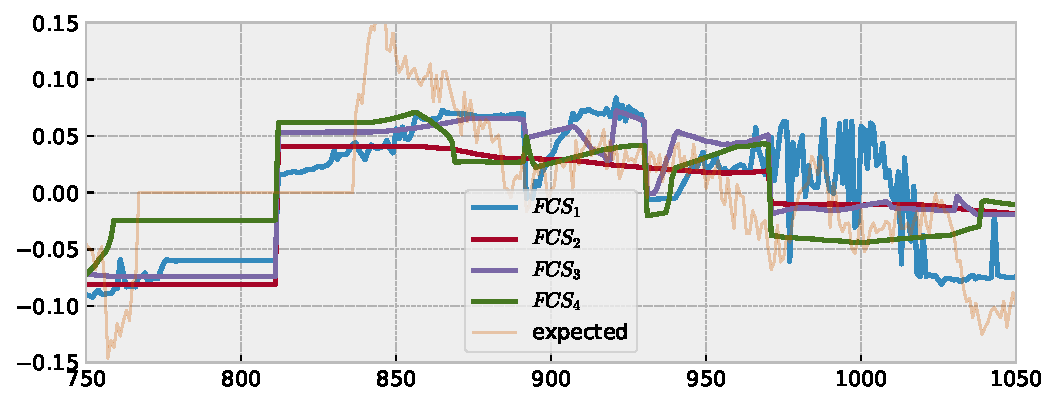
\includegraphics[width=\textwidth]{lm-fcs-outs-all-test-comparison-detail}}
	\caption[Comparación del perfil de aceleración real y el inferido por los modelos entrenados]{Comparación del perfil de aceleración real y el inferido por los modelos entrenados. En la visión general se puede observar el perfile real en color semi-transparente. Debajo, en el perfil, se amplía una pequeña sección del perfil para mostrar los diferentes ajustes de los modelos entrenados y cómo difieren del valor real.}
	\label{fig:fcs-test-comparisons}
\end{figure}

En el detalle podemos ver cómo se ajusta el controlador con menor error en test frente al resto. Mientras que el $FCS_1$ presenta picos de variación que aproximan el valor inferido al valor real, el resto de controladores mantiene valores constantes separados en escalones.

\section{Modelo basado en \acrlongplsp{mlp}\index{perceptron multicapa}}

Para determinar el modelo óptimo de \acrlongsp{mlp}\index{perceptron multicapa} en comportamiento longitudinal, se han realizado entrenamientos sobre arquitecturas con diferente cantidad de neuronas y capas ocultas.

Las arquitecturas más ilustrativas de todas las probadas se resumen en la tabla~\ref{tbl:cf-mlp-architectures}.

\begin{table*}
	\centering
	\caption[Resumen de las arquitecturas de \acrlongplsp{mlp} para el modelo longitudinal][2em]{Resumen de las arquitecturas de de \acrlongplsp{mlp} para el modelo longitudinal. La posición de cada número de la topología indica el índice de la capa oculta y su valor el número de nodos (neuronas) que incluye dicha capa. Las arquitecturas seleccionadas en esta tabla son aquellas consideradas relevantes tras un proceso manual de ensayo y error.}
	\label{tbl:cf-mlp-architectures}
	\begin{tabularx}{\linewidth}{YYYYYY}
		\toprule
		\multirow{2}{*}{} & \multirow{2}{*}{Topología} & \multirow{2}{*}{Epochs} & \multicolumn{3}{c}{RMS} \\
		& & & Entrenamiento & Validación & Test \\
		\midrule
		\rowcolor{black!20} $MLP_1$ & $16$        & $10^5$ & $0.057$ & $0.057$ & $0.069$  \\
		$MLP_2$ & $8, 2$      & $10^5$ & $0.061$ & $0.061$ & $0.056$  \\
		\rowcolor{black!20} $MLP_3$ & $16, 8$     & $10^5$ & $0.051$ & $0.051$ & $0.060$  \\
		$MLP_4$ & $16, 16, 8$ & $10^5$ & $0.046$ & $0.046$ & $0.061$  \\
		\bottomrule
	\end{tabularx}
\end{table*}

El modelo de funciones de activación que se ha utilizado es de tipo tangente hiperbólica en todas las neuronas salvo en la última, que se ha utilizado una activación lineal. En pruebas previas a la selección de estas funciones de activación se han utilizado también funciones de activación de tipo \acrshort{relu}\index{ReLU}, pero las tasas de error tras el entrenamiento eran notablemente más altas por lo que se ha optado al final por el uso de activación basada en tangente hiperbólica. Los pesos de la red han sido inicializados con una muestra aleatoria uniforme de valores reales en el intervalo $(-0.25, 0.25)$.

La Figura~\ref{fig:lm-mlp-rmse-all-comparisons} muestra la evolución del \gls{rmse} durante el proceso de entrenamiento. También se ilustra el error de test durante el mismo, aunque éste no se ha utilizado para decidir las arquitecturas y es simplemente informativo.

\begin{figure}
	\centering
	\subfloat[Entrenamiento y validación]{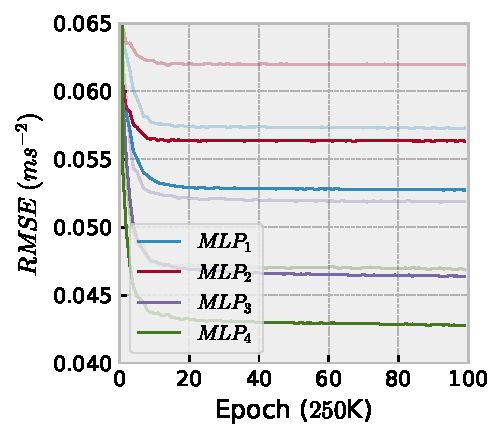
\includegraphics[width=.45\textwidth]{lm-mlp-rmse-all-training-and-validation-detail}}\qquad
	\subfloat[Test]{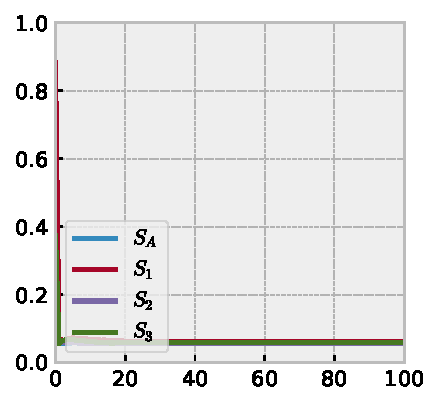
\includegraphics[width=.45\textwidth]{lm-mlp-rmse-all-test-detail}}
	\caption[Evolución del error durante el entrenamiento en las arquitecturas de \acrshort{mlp} para el modelo longitudinal]{Visión en detalle de la evolución del error en los conjuntos de entrenamiento y validación (izquierda) y de test (derecha). Para cada arquitectura, el color más transparente se corresponde al error en el conjunto de validación. El error de test se muestra debido a que nos ofrece puede ofrecer intuición de qué forma aprende la red, pero su evolución no se ha considerado para determinar las arquitecturas.}
	\label{fig:lm-mlp-rmse-all-comparisons}
\end{figure}

Estos errores se encuentran entre los \SI{0.05}{\metre\per\square\second} y los \SI{0.07}{\metre\per\square\second}, lo cual consideramos que es una aproximación aceptable. Una particularidad del problema ha sido la inestabilidad de los entrenamientos, esto es, la alta sensibilidad a los valores de inicialización de los parámetros. La intuición tras ver la evolución de los entrenamientos es que la función de error sufre de muchos mínimos locales o mesetas.

Una visión de detalle del ajuste de estas arquitecturas al conjunto de test se puede ver en la figura~\ref{fig:cf-mlp-test-comparisons}, donde se muestra el perfil de aceleración del conjunto de test y los perfiles de aceleración de las redes entrenadas.

\begin{figure}
	\centering
	\subfloat[Perfil completo]{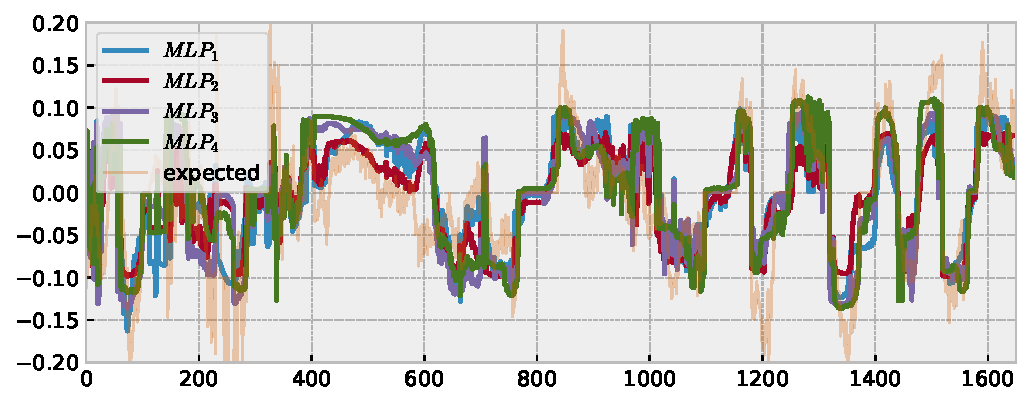
\includegraphics[width=\textwidth]{lm-mlp-outs-all-test-comparison}}\qquad
	\subfloat[Detalle entre frames de $750$ a $1050$]{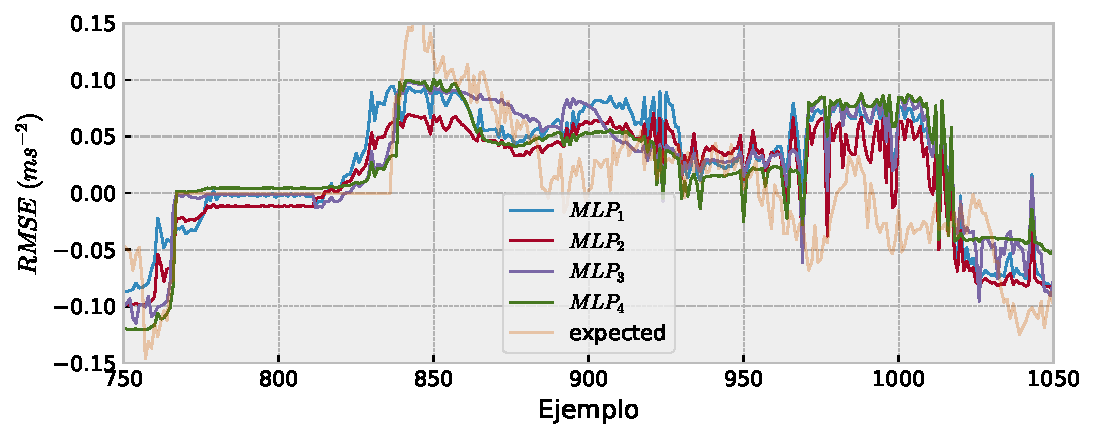
\includegraphics[width=\textwidth]{lm-mlp-outs-all-test-comparison-detail}}
	\caption[Comparación del perfil de aceleración real y el inferido por los modelos entrenados]{Comparación del perfil de aceleración real y el inferido por los modelos entrenados. En la visión general se puede observar el perfil real en semi-transparente. En el detalle, se amplía una pequeña sección del perfil para mostrar los diferentes ajustes de los modelos entrenados y cómo difieren del valor real.}
	\label{fig:cf-mlp-test-comparisons}
\end{figure}

Al contrastar los errores de test, podemos determinar que la arquitectura que mejor generaliza es la $MLP_2$, hecho que se confirma en el ajuste de los perfiles de aceleración. Por lo tanto, parece razonable elegir el modelo $MLP_2$ como candidato para la representación del modelo longitudinal de los conductores.

\section{Comparación entre modelos}

Las mejores arquitecturas de ambos modelos han sido la $MLP_2$ para los \acrlongplsp{mlp}\index{perceptron multicapa} y $FCS_1$ para los \acrlongplsp{fcs}\index{sistema de control borroso}. Los errores y el perfil de aceleración para ambos modelos se muestran en la Figura~\ref{fig:cf-comparison-between-best-mlp-and-fcs-architecture}.

\begin{figure}
	\centering
	\subfloat[Error en test]{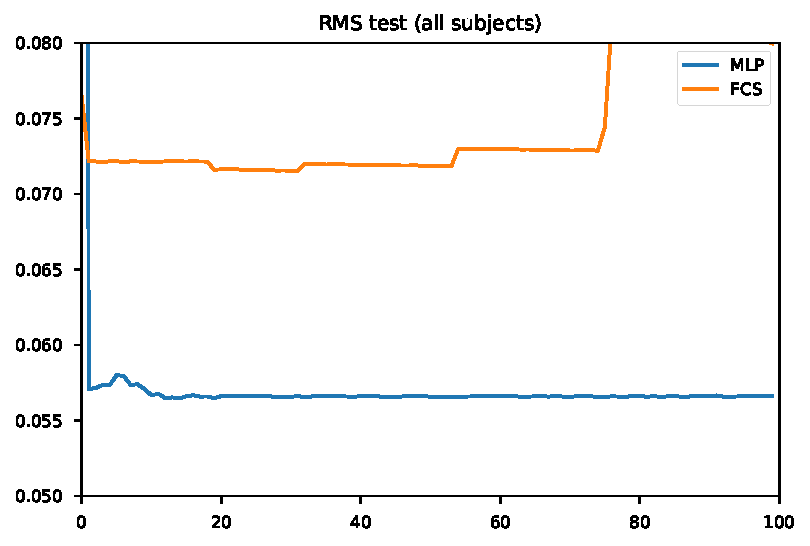
\includegraphics[width=.46\textwidth]{comparison-between-best-mlp-and-fcs-architecture-rms}}\qquad
	\subfloat[Perfil de aceleración]{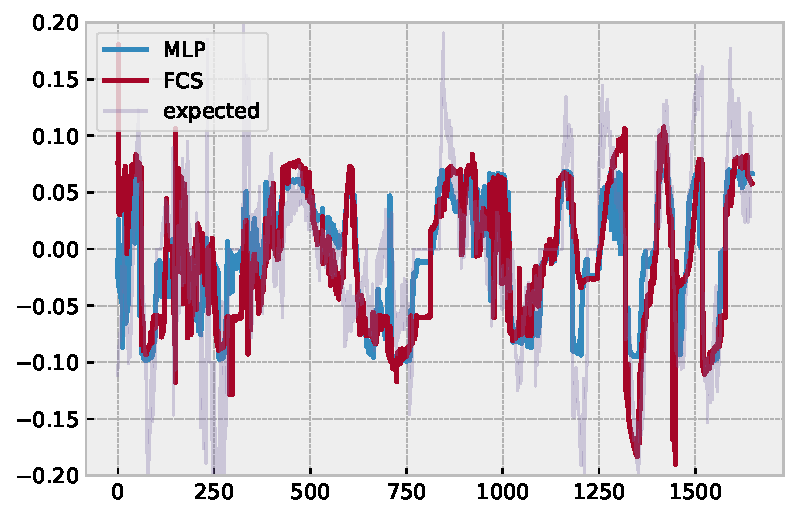
\includegraphics[width=.46\textwidth]{comparison-between-best-mlp-and-fcs-architecture-acceleration-profile}}
	\caption[Comparación entre los dos tipos de modelo longitudinal]{Comparación de la mejor arquitectura de \acrlongplsp{mlp} frente a la mejor arquitectura de \acrlongplsp{fcs}: (a) diferencia entre los errores cuadráticos medios de ambas arquitecturas y (b) perfiles de aceleración en el conjunto de test.}
	\label{fig:cf-comparison-between-best-mlp-and-fcs-architecture}
\end{figure}

Aunque el modelo basado en \acrlongplsp{fcs}\index{sistema de control borroso} arroja un error bajo en test, y además tiende a ajustarse al perfil de aceleración, parece que el problema es suficientemente complejo como para no poder representarse como un simple \acrlongsp{fcs}\index{sistema de control borroso}.

Además, el error arrojado por el \acrlongsp{mlp}\index{perceptron multicapa} es sustancialmente menor y, por tanto, la arquitectura elegida para el modelo longitudinal será la $MLP_2$.

\section{Modelos longitudinales específicos}

La arquitectura seleccionada se ha usado para generar los modelos de cada uno de los conductores por separado para comprobar que (i) los errores y precisiones se mantienen en el orden del modelo global, y (ii) los modelos capturan las particularidades de cada sujeto de estudio.

En la Figura~\ref{fig:lm-specific-training-validation-and-test-comparison} se muestra la evolución del \gls{rmse}\index{RMSE} en test para cada uno de los sujetos tras entrenar los modelos de arquitectura $MLP_2$ con los datos de los sujetos.

\begin{figure}
	\centering
	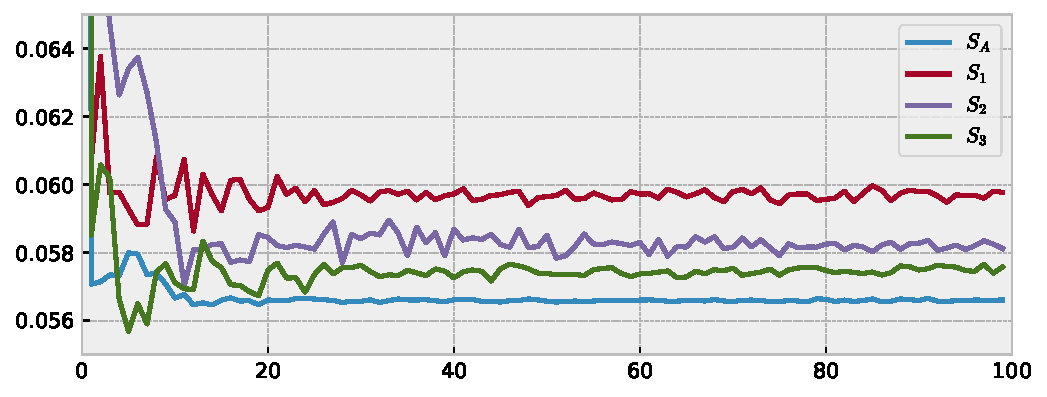
\includegraphics[width=\textwidth]{lm-specific-rmse-all-test-detail}
	\caption[Comparativa de la evolución del \gls{rmse} en test para los sujetos de la arquitectura seleccionada para el modelo longitudinal]{Comparativa de la evolución del error de test entre los sujetos de la arquitectura seleccionada para el modelo longitudinal. El \gls{rmse} en test en el caso del sujeto $S_2$ es muy alto (mayor que $0.2$) comparado con el error en el resto de sujetos y en el global.}
	\label{fig:lm-specific-training-validation-and-test-comparison}
\end{figure}

Se puede observar que el error en test de los sujetos es ligeramente mayor que el del conjunto global. Esto se puede explicar por la mayor capacidad de generalización de $S_A$ al haber sido entrenado con un conjunto de datos mayor.

Los errores se resumen en la Tabla~\ref{tbl:lm-specific-rmse}. Sin embargo, se mantienen aproximadamente dentro del mismo rango de error que el modelo global.

\begin{table}
	\centering
	\caption[Resumen de los valores de \Acrshort{rmse} para los modelos específicos de comportamiento longitudinal]{Resumen de los valores de \Acrshort{rmse} para los modelos específicos de comportamiento longitudinal.}
	\label{tbl:lm-specific-rmse}
	\begin{tabularx}{\linewidth}{YYYYYY}
		\toprule
		\multirow{2}{*}{} & \multicolumn{3}{c}{\ac{rmse}}      \\ 
		& Entrenamiento & Validación & Test \\
		\midrule
		\rowcolor{black!20} $S_A$ & $0.056$ & $0.062$ & $0.057$  \\
		$S_1$ & $0.045$ & $0.039$ & $0.060$  \\
		\rowcolor{black!20} $S_2$ & $0.048$ & $0.047$ & $0.058$  \\
		$S_3$ & $0.055$ & $0.054$ & $0.058$  \\
		\bottomrule
	\end{tabularx}
\end{table}

Para verificar que esta topología es capaz de capturar las diferencias entre conductores, podemos comprobar los perfiles de aceleración específicos de los conductores en la Figura~\ref{fig:lm-subjects-comparison}.

\begin{figure}
	\centering
	\subfloat[Sujeto $S_1$]{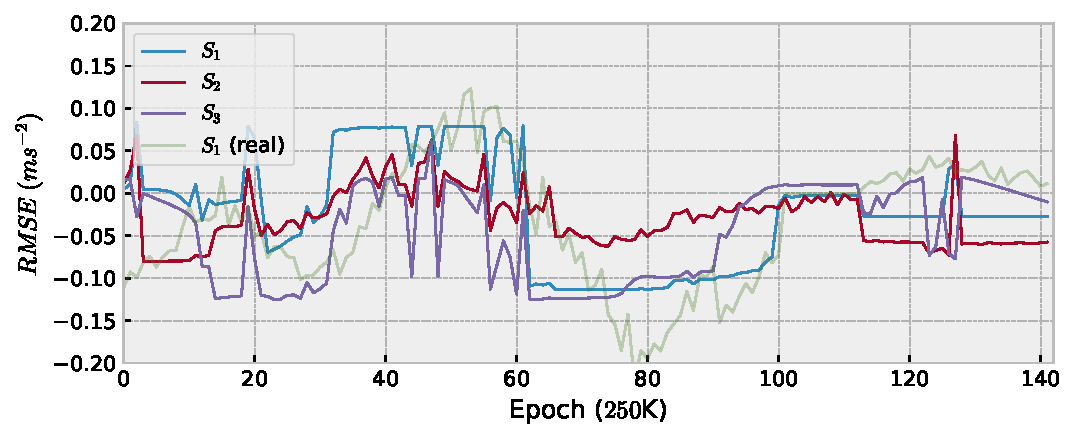
\includegraphics[width=\textwidth]{lm-subjects-comparison-with-edgar-acceleration-profiles}}\qquad
	\subfloat[Sujeto $S_2$]{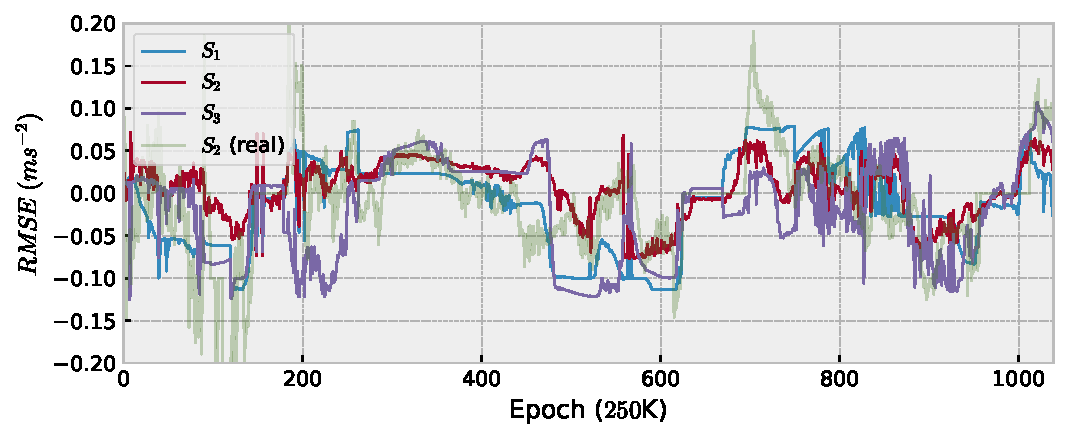
\includegraphics[width=\textwidth]{lm-subjects-comparison-with-jj-acceleration-profiles}}\qquad
	\subfloat[Sujeto $S_3$]{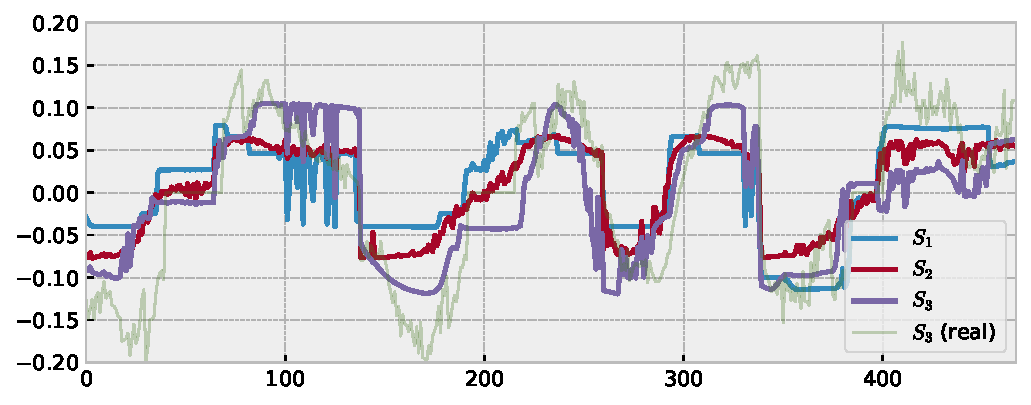
\includegraphics[width=\textwidth]{lm-subjects-comparison-with-miguel-acceleration-profiles}}
	\caption[Diferencia entre los perfiles de aceleración para los diferentes sujetos]{Diferencia entre los perfiles de aceleración para los diferentes sujetos.}
	\label{fig:lm-subjects-comparison}
\end{figure}

En la figura se muestra gráficamente el perfil de aceleración de cada uno de los conductores sobre cada uno de los perfiles reales. Podemos observar que, para cada uno de los perfiles de aceleración, los de los sujetos originales se aproximan más a sus respectivos perfiles que los del resto. En la Tabla~\ref{tbl:lm-subjects-comparison} se describen los \acrshort{rmse}\index{RMSE} cruzados para de cada uno de los conductores.

\begin{table}
	\centering
	\caption[Comparación de los errores de aceleración en los diferentes modelos longitudinales]{Comparación de los errores de aceleración en los diferentes modelos longitudinales. Las filas se corresponden con los recorridos mientras que las columnas se corresponden con los modelos que se han intentado ajustar a ellas.}
	\label{tbl:lm-subjects-comparison}
	\begin{tabularx}{\linewidth}{YYYY}
		\toprule
		& $S_1$ & $S_2$ & $S_3$ \\
		\midrule
		\rowcolor{black!20} $S_1$ & $0.059$        & $0.074$        & $0.070$ \\
		$S_2$ & $0.064$        & $0.058$        & $0.067$ \\
		\rowcolor{black!20} $S_3$ & $0.065$        & $0.065$        & $0.057$ \\
		\bottomrule
	\end{tabularx}
\end{table}

Se observa que el \acrshort{rmse}\index{RMSE} es menor cuando el modelo de conductor se aplica sobre los datos del conjunto de test de sus respectivos conductores.

Estos modelos basados en la arquitectura $MLP_2$ serán los comportamientos longitudinales de los sujetos en el simulador. Veremos su desempeño en el capítulo \nameref{ch:simulation-implementation}.